\documentclass[11pt]{article}
\usepackage[margin=1in]{geometry} 
\usepackage{amsmath,amsthm,amssymb,amsfonts}
\usepackage[utf8]{inputenc}
\usepackage[T1]{fontenc}
\usepackage{microtype}
\usepackage{mathpazo}
\usepackage{euler}
\usepackage{xcolor}
\usepackage{tikz}
\usepackage{tikz-cd}
\usetikzlibrary{arrows}
\usetikzlibrary{matrix}
\usepackage{fancyhdr}
\pagestyle{fancy}
\usepackage{enumitem}

\newcommand{\N}{\mathbb{N}}
\newcommand{\Z}{\mathbb{Z}}
\newcommand{\Q}{\mathbb{Q}}
\newcommand{\R}{\mathbb{R}}
\newcommand{\C}{\mathbb{C}}
\newcommand{\Ss}{\mathbb{S}}
\newcommand{\M}[2]{\mathsf{M}_{#1}#2}
\newcommand{\X}{\mathfrak{X}}
\renewcommand{\div}{\operatorname{div}}
\newcommand{\grad}{\operatorname{grad}}
\newcommand{\im}{\operatorname{im}}
\newcommand{\eps}{\varepsilon}
\newcommand{\dpart}[2]{\frac{\partial#1}{\partial#2}}
\newcommand{\nat}[1]{[\![#1]\!]}
\newcommand{\natzero}[1]{\nat{#1}_0}
\newcommand{\adj}[1]{\operatorname{adj}(#1)}
\newcommand{\ip}[1]{\langle #1 \rangle}
\newcommand{\ol}{\overline}
\newcommand{\hook}[3]{\frac{\partial}{\partial x_{#1}}\Big\rvert_{#2}^{#3}}
\usepackage{rotating}
\newcommand*{\isoarrow}[1]{\arrow[#1,"\rotatebox{90}{\LARGE{\(\sim\)}}"
]}
\renewcommand{\d}{\operatorname{d}}
\definecolor{color}{RGB}{80, 117, 73}
\newcommand{\paint}[1]{\color{color}{#1}}

\renewcommand*{\proofname}{\paint{Demostraci\'on}}
\newenvironment{theorem}[2][Teorema]{\begin{trivlist}
\item[\hskip \labelsep \paint{{\bfseries #1}}\hskip \labelsep {\bfseries #2.}]}{\end{trivlist}}
\newenvironment{lemma}[2][Lema]{\begin{trivlist}
\item[\hskip \labelsep \paint{{\bfseries #1}}\hskip \labelsep {\bfseries #2.}]}{\end{trivlist}}
\newenvironment{exercise}[2][Ejercicio]{\begin{trivlist}
\item[\hskip \labelsep \paint{{\bfseries #1}}\hskip \labelsep {\bfseries #2.}]}{\end{trivlist}}
\newenvironment{obs}[2][Observaci\'on]{\begin{trivlist}
\item[\hskip \labelsep \paint{{\bfseries #1.}}]}{\end{trivlist}}
\newenvironment{reflection}[2][Resoluci\']{\begin{trivlist}
\item[\hskip \labelsep {\bfseries #1}\hskip \labelsep {\bfseries #2.}]}{\end{trivlist}}
\newenvironment{proposition}[2][Proposici\'on]{\begin{trivlist}
\item[\hskip \labelsep \paint{{\bfseries #1}}\hskip \labelsep {\bfseries #2.}]}{\end{trivlist}}
\newenvironment{corollary}[2][Corolario]{\begin{trivlist}
\item[\hskip \labelsep {\bfseries #1}\hskip \labelsep {\bfseries #2.}]}{\end{trivlist}}

%-----------------------

\title{
\LARGE{\paint{Geometr\'ia Diferencial}}
\\
\vspace{0.5pt}
\small{\paint{Ejercicios para Entregar - Pr\'acticas 5 y 6}}
}
\author{\paint{Guido Arnone}}
\date{}
\lhead{Guido Arnone}
\rhead{Pr\'actica 5}

\begin{document}

\maketitle

\begin{center}
\paint{\large{Sobre los Ejercicios}}
\end{center}

\begin{center}
Elegí los ejercicios $\paint{(5)}$ y $\paint{(7)}$ de la práctica cinco, y el ejercicio $\paint{(9)}$ de la práctica seis.
$\paint{
\rule{400pt}{0.5pt}
}$
\vspace{35pt}
\end{center}

\begin{exercise}{5}Sea $M$ una variedad compacta y sin borde de dimensión $n$. Probar que si
$\omega\in\Omega^n(M)$ es una forma de volumen, entonces $\omega$ no es exacta.
\end{exercise}
\begin{proof} Supongamos que $\omega$ es exacta, y sea entonces $\eta \in \Omega^{n-1}(M)$ tal que $d\eta= \omega$. Por el teorema de Stokes es
\begin{align*}
\int_M\omega = \int_M d\eta = \int_{\partial M}i^*(\eta) = 0,
\end{align*}
ya que $M$ no tiene borde. Sin embargo, esto es absurdo: como $\omega$ es una forma de volumen y $M$ es compacta, su integral da un valor real no nulo. Vemos así que $\omega$ no puede ser exacta.
\end{proof}

\begin{exercise}{7} Si $M$ es una variedad compacta, orientada y con borde, no existe una retracción diferenciable $M \to \partial M$.
\end{exercise}
\begin{proof} Supongamos que $r : M \to \partial M$ es una retracción, es decir, que
\begin{center}
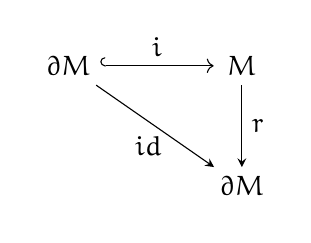
\begin{tikzpicture}
  \matrix (m) [matrix of math nodes,row sep=3em,column sep=4em,minimum width=2em]
  {
     \partial M & M\\
      & \partial M\\};
  \path[-stealth]
    (m-1-1) edge [right hook->] node [above] {$i$} (m-1-2)
    (m-1-1) edge node [below] {$id \ \ $} (m-2-2)
    (m-1-2) edge node [right] {$r$} (m-2-2);
\end{tikzpicture}
\end{center}
conmuta. 

Como para cada $q \in \N_0$ la asignación
\begin{align*}
\Omega^q : \ &\mathsf{Man} \longrightarrow \mathsf{Vect}_\R\\
&M \longmapsto \Omega^q(M)\\
&\downarrow_{f} \ \longmapsto \quad \uparrow_{f^*}\\
&N \longmapsto \Omega^q(N)
\end{align*}
es funtorial contravariante, el diagrama
\begin{center}
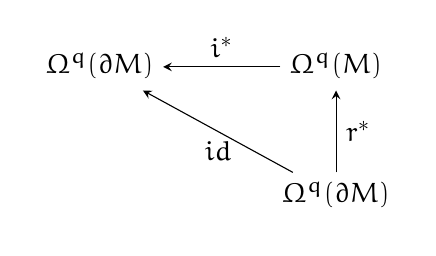
\begin{tikzpicture}
  \matrix (m) [matrix of math nodes,row sep=3em,column sep=4em,minimum width=2em]
  {
     \Omega^q(\partial M) & \Omega^q(M)\\
      & \Omega^q(\partial M)\\};
  \path[-stealth]
    (m-1-2) edge [right] node [above] {$i^*$} (m-1-1)
    (m-2-2) edge node [below] {$id$} (m-1-1)
    (m-2-2) edge node [right] {$r^*$} (m-1-2);
\end{tikzpicture}
\end{center}
conmuta. Es decir, para cualquier $q$-forma $\omega$ de $\partial M$ se tiene que \begin{align}
i^*r^*(\omega) = \omega.
\end{align}

Dado que $M$ es orientable, así lo es su borde, y por lo tanto existe una $(n-1)$-forma de volumen $\eta \in \Omega^{n-1}(\partial M)$. Sabemos además que $d\eta = 0$ pues esta última es una $n$-forma y $\partial M$ tiene dimensión $n-1$. En particular, la forma $dr^*(\eta) = r^*(d\eta) = r^*(0) = 0$ integra cero sobre $\partial M$. 

Usando $\paint{(1)}$ y el teorema de Stokes vemos que
\begin{align*}
0 = \int_M dr^*(\eta) = \int_{\partial M}i^*r^*(\eta) = \int_{\partial M} \eta
\end{align*}
lo cual es una contradicción: como $\partial M$ es compacta (ya que $M$ lo es y $\partial M$ es cerrado) y $\eta$ es una forma de volumen, su integral sobre $\partial M$ existe y es no nula. 

Como el absurdo partió de suponer que $r$ existía, concluimos que no puede haber una retracción diferenciable de $M$ a su borde.
\end{proof}

\begin{center}
$\paint{
\rule{400pt}{0.5pt}
}$
\vspace{10pt}
\end{center}

\begin{lemma}{1} Sea $M$ una variedad riemanniana orientada y compacta, y notemos $dV$ al elemento de volumen riemanniano. Si tomamos un campo $X \in \X(M)$ y $u \in C^\infty(M)$, entonces
\begin{itemize}[listparindent = \parindent]
\item[i)] $\iota_{uX}(dV) = u\iota_X(dV)$
\item[ii)] $du \wedge \iota_X(dV) = \ip{\grad(u), X}dV$.
\end{itemize}
\end{lemma}
\begin{proof} Hacemos cada inciso por separado.
\begin{itemize}[listparindent = \parindent]
\item[i)] Efectivamente, si $p \in M$ y $v_1, \dots, v_{n-1} \in T_pM$ entonces
\begin{align*}
\iota_{uX}(dV)_p(v_1, \dots, v_{n-1}) &= dV_p(u(p)X_p,v_1, \dots, v_{n-1}) = u(p)dV_p(X_p,v_1,\dots,v_{n-1})\\
&= u(p)\iota_X(dV)_p(v_1,\dots,v_{n-1}) = (u\iota_X(dV))_p(v_1, \dots, v_{n-1}).
\end{align*}
\item[ii)] Basta ver la igualdad al evaluar en cada punto $p\in M$ y vectores $v_1, \dots, v_{n} \in T_pM$. Más aún, alcanza hacerlo para una base del espacio tangente. 

Dado que $M$ posee una métrica riemanniana y trabajaremos con el elemento de volumen riemanniano, vamos a suponer sin pérdida de generalidad que los vectores $v_1, \dots, v_{n}$ forman una base ortonormal de $T_pM$ orientada positivamente. De esta forma, resulta $dV_p(v_1, \dots, v_n) = 1$. Ahora sí, evaluando es
\begin{align*}
(du \wedge \iota_X(dV))_p(v_1,\dots,v_n) &= \frac{1}{n-1!}\sum_{\sigma \in \Ss_{n}}(-1)^\sigma \sigma \cdot (du \otimes \iota_X(dV))_p(v_1, \dots, v_n)\\
&= \frac{1}{n-1!}\sum_{\sigma \in \Ss_{n}}(-1)^\sigma d_pu(v_{\sigma(1)}) \otimes dV_p(X_p,v_{\sigma(2)}, \dots, v_{\sigma(n)}).
\end{align*}

Como los vectores $v_1, \dots, v_n$ son una base ortonormal de $T_pM$, el vector tangente $X_p$ se escribe como
\begin{align*}
X_p = \sum_{j=1}^n \ip{X_p,v_j}v_j
\end{align*}
donde $\ip{X_p,v_j}$ es el producto interno en $T_pM$ inducido por la métrica. Como $dV$ es multilineal y anstisimétrica, se anula en vectores linealmente dependientes. Por lo tanto, tenemos que
\begin{align*}
dV_p(X_p,v_{\sigma(2)}, \dots, v_{\sigma(n)}) &= \sum_{j=1}^n \ip{X_p,v_j}dV_p(v_j,v_{\sigma(2)}, \dots, v_{\sigma(n)})\\
& = \ip{X_p,v_{\sigma(1)}}dV_p(v_{\sigma(1)},v_{\sigma(2)}, \dots, v_{\sigma(n)}).
\end{align*}

Volviendo a la igualdad anterior, obtenemos
\begin{align*}
(du \wedge \iota_X(dV))_p(v_1,\dots,v_n) &= \frac{1}{n-1!}\sum_{\sigma \in \Ss_{n}}(-1)^\sigma \sigma \cdot (du \otimes \iota_X(dV))_p(v_1, \dots, v_n)\\
&= \frac{1}{n-1!}\sum_{\sigma \in \Ss_{n}}(-1)^\sigma d_pu(v_{\sigma(1)}) \otimes \ip{X_p,v_{\sigma(1)}}dV_p(v_{\sigma(1)},v_{\sigma(2)}, \dots, v_{\sigma(n)})\\
&= \frac{1}{n-1!}\sum_{\sigma \in \Ss_{n}}(-1)^\sigma d_pu(v_{\sigma(1)}) \otimes \ip{X_p,v_{\sigma(1)}}(-1)^\sigma dV_p(v_1,v_2, \dots, v_n)\\
&= \frac{1}{n-1!}\sum_{\sigma \in \Ss_{n}}\ip{X_p,v_{\sigma(1)}}d_pu(v_{\sigma(1)}) \otimes dV_p(v_1,v_2, \dots, v_n)\\
&= \frac{1}{n-1!}\sum_{\sigma \in \Ss_{n}}\ip{X_p,v_{\sigma(1)}}d_pu(v_{\sigma(1)}) = \sum_{j=1}^n\ip{X_p,v_j}d_pu(v_j)\\
&= d_pu\left(\sum_{j=1}^n\ip{X_p,v_j}v_j\right) = d_pu(X_p) = \ip{\grad_p(u),X_p}.
\end{align*}
 
Usando una vez más que $dV_p(v_1, \dots, v_n) = 1$, tenemos finalmente que
\begin{align*}
(du \wedge \iota_X(dV))_p(v_1,\dots,v_n) &= \ip{\grad_p(u),X_p} \cdot 1\\
&= \ip{\grad_p(u),X_p}dV_p(v_1, \dots, v_n)\\
& = (\ip{\grad(u),X}dV)_p(v_1, \dots, v_n).
\end{align*}
\end{itemize}
\end{proof}
\newpage
\begin{exercise}{9}Sea $M$ una variedad riemanniana orientada y $dV$ su elemento de
volumen riemanniano. Si $X \in \X(M)$ es un campo sobre $M$,
llamamos \emph{divergencia} de $X$ a la función $\div(X)$ tal que
  \[
  d(i_X(dV)) = \div(X)\cdot dV.
  \]
Obtenemos de esta forma una función $\div:\X(M)\to C^\infty(M)$.
\begin{itemize}[listparindent = \parindent]
\item[a)] Si $M$ es compacta, para cada $X\in\X(M)$ se tiene que
  \[
  \int_M\div(X)\cdot dV = \int_{\partial M}\ip{X,N}\cdot d\tilde{V},
  \]
con $N$ la normal unitaria interior a $\partial M$ y $d\tilde V$ el
elemento de volumen riemanniano sobre $\partial M$ correspondiente a la
métrica inducida por la de $M$.

\item[b)] Si $u\in C^\infty(M)$ y $X\in\X(M)$, entonces
  \[
  \div(uX) = u\cdot\div(X) + \ip{\grad(u),X}.
  \]
y deducir la fórmula de integración por partes
  \[
  \int_M\ip{\grad(u),X}\cdot dV  
        = -\int_M u\cdot\div(X)\cdot dV
          +\int_{\partial M}u\ip{X,N}\cdot d\tilde V.
  \]
\end{itemize}  
\end{exercise}
\begin{proof} Hacemos cada inciso por separado.
\begin{itemize}[listparindent = \parindent]
\item[a)] Sea $M$ una variedad compacta y $X \in \X(M)$. Notemos en primer lugar que por el teorema de Stokes es
\begin{align*}
\int_M\div(X) \cdot dV = \int_M d(\iota_X(dV)) = \int_{\partial M} i^*(\iota_X(dV))
\end{align*}
así que bastaría ver que $i^*(\iota_X(dV)) =  \ip{X,N}\cdot d\tilde{V}$. Veamos la igualdad para cada $p \in \partial M$ y $v_1,\dots, v_{n-1} \in T_p \partial M$. 

Como las $(n-1)$-formas son funciones multilineales antisimétricas, al evaluarlas en conjuntos linealmente dependientes siempre valen cero. Por lo tanto, podemos asumir que $\{v_i\}_{1 \leq i \leq n-1}$ es un conjunto linealmente independiente, y como $\dim \partial M = n-1$, resulta una base.

En consecuencia los \textit{pushforwards } $\{d_pi(v_i)\}_{1 \leq i \leq n-1}$ por la inclusión $i : \partial M \to M$ son un conjunto linealmente independiente de $T_pM$. Por definición del campo normal $N$, agregando $N_p$ podemos completar estos a una base $B = \{N_p, d_pi(v_1), \dots, d_pi(v_{n-1})\}$. Recordemos también que por definición es 
\begin{align}
d\tilde{V}_p(v_1, \dots, v_{n-1}) = i^*(\iota_N(dV))_p(v_1, \dots, v_{n-1}) = dV_p(N_p,d_pi(v_1), \dots, d_pi(v_{n-1})).
\end{align}

Ahora, dado que $B$ es base de $T_pM$, el vector tangente $X_p$ tiene una escritura única como combinación lineal de los vectores de $V$,
\begin{align*}
X_p = \alpha N_p + \sum_{j=1}^{n-1}\beta_j d_pi(v_j).
\end{align*}

A partir de la multilinealidad de $dV$ y usando la una vez más que las formas se anulan en conjuntos linealmente dependientes, se tiene que 
\begin{align*}
i^*(\iota_X(dV))_p(v_1, \dots, v_{n-1}) &= \iota_X(dV)_p(d_pi(v_1), \dots, d_pi(v_{n-1}))\\
&= dV_p(X_p,d_pi(v_1), \dots, d_pi(v_{n-1}))\\
&= dV_p\left(\alpha N_p + \sum_{j=1}^{n-1}\beta_j d_pi(v_j),d_pi(v_1), \dots, d_pi(v_{n-1})\right)\\
&= \alpha dV_p\left(N_p,d_pi(v_1), \dots, d_pi(v_{n-1})\right).
\end{align*}

Más aún, como $N_p$ es unitario y ortogonal a $d_pi(v_1), \dots, d_pi(v_{n-1})$, es
\begin{align*}
\ip{X_p,N_p} &= \left\ip{\alpha N_p + \sum_{j=1}^{n-1}\beta_j d_pi(v_j), N_p\right}\\
&= \alpha\ip{N_p,N_p}+ \sum_{j=1}^{n-1}\beta_j \ip{N_p,d_pi(v_j)} = \alpha\ip{N_p,N_p} = \alpha.
\end{align*}

En definitiva, usando $\paint{(2)}$ obtenemos
\begin{align*}
i^*(\iota_X(dV))_p(v_1, \dots, v_{n-1}) &= \ip{X_p,N_p}dV_p\left(N_p,d_pi(v_1), \dots, d_pi(v_{n-1})\right)\\
&= \ip{X_p,N_p}d\tilde{V}_p(v_1, \dots, v_{n-1}).
\end{align*}

Como esto es cierto para cada punto $p \in \partial M$ y elección de vectores $v_1, \dots, v_{n-1} \in T_p \partial M$, resulta $i^*(\iota_X(dV)) = \ip{X,N}d\tilde{V}$, que es lo que queríamos probar.
\item[b)] Notemos en primer lugar que, en vista del $\paint{\text{Lema $1$}}$, es
\begin{align*}
div(uX)dV &= d(\iota_{uX}(dV)) = d(u\iota_{X}(dV)) = du \wedge \iota_X(dV) + (-1)^0 u \wedge d(\iota_X(dV))\\
&= \ip{\grad(u),X}dV + u\div(X)dV = (\ip{\grad(u),X}+ u\div(X))dV.
\end{align*}
Si tomamos $p \in M$ y $v_1, \dots, v_n \in T_pM$ una base ortonormal orientada positivamente, evaluando vemos que
\begin{align*}
div(uX)_p = \ip{\grad_p(u),X_p}+ u(p)\div(X)_p
\end{align*}
y por lo tanto, efectivamente resulta
\begin{align*}
div(uX) = \ip{\grad(u),X}+ u\div(X).
\end{align*}
Ahora integrando y usando el ítem $\paint{(a)}$ es
\begin{align*}
\int_{\partial M}u\ip{X,N} d\tilde{V} &= \int_{\partial M}\ip{uX,N} d\tilde{V} = \int_{M}\div(uX)dV= \int_M\ip{\grad(u),X}dV+ u\div(X)dV\\
& = \int_M\ip{\grad(u),X}dV+ \int_M u\div(X)dV.
\end{align*}
Restando llegamos a la identidad de «integración por partes»,
\begin{align*}
\int_M\ip{\grad(u),X} dV  
        = -\int_M u\cdot\div(X) dV
          +\int_{\partial M}u\ip{X,N} d\tilde V.
\end{align*}
\end{itemize}
\end{proof}


\end{document}
